\documentclass[]{article}
\usepackage{graphicx}

%opening
\title{YJFC Armory App - Equipment Checkout}
\author{Susanna Dong}

\begin{document}

\maketitle

\begin{abstract}
tl;dr This is the guide for equipment checkout.
\end{abstract}

\section{Instructions}
Screenshot of application

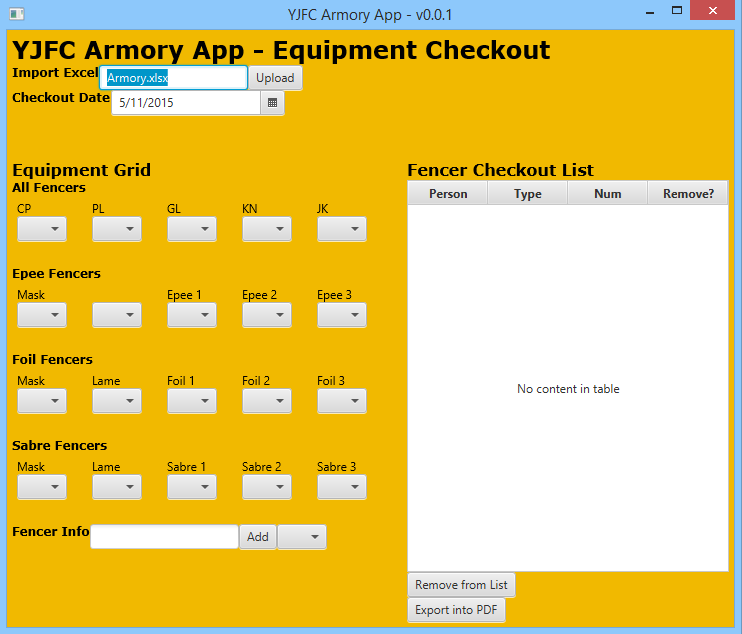
\includegraphics[scale=0.7]{screen.png}

\begin{itemize}
\item \textbf{Import Excel}: Input a valid filepath to an Excel spreadsheet. The Excel spreadsheet format must be .xlsx. Press 'Upload' to upload the spreadsheet into main memory.

\item \textbf{Checkout Date}: Date of checkout. Determines file name of PDF file.

\item \textbf{Equipment Grid}: Grid of equipment filled in with data from Excel spreadsheet.

\item \textbf{Fencer Info}: Two options. Typing in a fencer's name, selecting the dropdown, and pressing 'Add' will associate all equipment to the fencer. Clicking the dropdown to the right of the button allows selection of fencers with existing equipment.

\item \textbf{Fencer Checkout List table}: displays all equipment checked out. Clicking the 'Removed' checkbox associated with the equipment and clicking 'Remove from List' will remove the fencer from the equipment.

\item \textbf{Export into PDF}: Exports the info displayed in the Fencer Checkout List into a PDF file.
\end{itemize}

\end{document}
